\chapter{Implementation and Evaluation}

\section{Wrapping MonPoly}

We opted to use Python as a programming language for our wrapper.
It is a powerful high level language that is widely used and has a large ecosystem of tools available.
While we tried to keep them to a minimum, some changes directly to MonPoly itself were necessary for the wrapper to work.

The wrapper code can be divided into two core parts.
The first part is responsible for providing the REST API endpoints and handling user input.
One might call this part the front end of the wrapper.
For this we use Flask \cite{Flask}, a lightweight web framework for Python.
It offers a convenient way of specifying the endpoints and handling web requests.

The second part handles the interactions with MonPoly and QuestDB.
One might call this the backend of the wrapper.

The distinction of these parts is reflected in the way we split the code into different files.
There are just three of them, in the "src" directory of the repository \cite{git-wrapper}.
The first one is "app.py" and it directly corresponds to the first part.
It is conventional to have a file called "app.py".
The "app.py" is to a Flask project, what a "main.py" file would be to regular python projects.
Both of these are however merely conventions.
Inside "app.py" there is one method for each REST API endpoint as described in the Architecture chapter.

The remaining two files, "monitor.py" and "db\_helper.py" correspond to the second part from above.
In "monitor.py" we define a "monitor" class, which is the heart of the wrapper.
During runtime there is always one single "monitor"- object, that keeps track of everything from the current signature, the current policy, how to reach QuestDB, to a potential MonPoly subprocess.
"db\_helper.py" is a small class, defining a "db\_helper" class that keeps track of the QuestDB configuration details, like ports, hostname, or the username.
The "monitor"- class has a "db\_helper"- object as a member.

The wrapper runs MonPoly as a subprocess and handles all interactions with MonPoly itself.
This subprocess is a member of the "monitor"- object and any interaction with the subprocess goes through this class.
Incoming events are first parsed and checked on some major formatting errors.
When the formatting is deemed acceptable the events get forwarded to MonPoly on a per time point basis.
If MonPoly reports an issue with a certain time stamp, either it is out of order or one event at that timestamp does not comply with the given signature, this time stamp gets ignored by MonPoly, and in turn the wrapper discards it as well.
If no issue is detected with a timestamp all events in at that timestamp get forwarded to the database.
Figure \ref{fig:flowchart} illustrates the control flow of this process.

In our implementation, one "monitor" object monitors one policy at any given time.
This policy can be changed, but never are there more than two policies being monitored.
An obvious extension, with many perceivable applications, would be to extend the wrapper to monitor multiple policies at the same time.
Multiple policies might be based on the same data, i.e. signature and it would thus be highly practical to monitor them in the same wrapper.
This would remove large redundancies if the identical data doesn't need to be stored multiple times in multiple databases.


\section{Policy Change}
% \tikzstyle{startstop} = [rectangle, rounded corners, 
minimum width=3cm, 
minimum height=1cm,
text centered, 
draw=black]
% fill=red!30]

\tikzstyle{io} = [trapezium, 
trapezium stretches=true, % A later addition
trapezium left angle=70, 
trapezium right angle=110, 
minimum width=3cm, 
minimum height=1cm, text centered, 
draw=black]
% , fill=blue!30]

\tikzstyle{process} = [rectangle, 
minimum width=3cm, 
minimum height=1cm, 
text centered, 
text width=3cm, 
draw=black] 
% fill=orange!30]

\tikzstyle{decision} = [diamond, 
minimum width=2cm, 
minimum height=1cm, 
text centered, 
text width=3cm,
draw=black]
% fill=green!30]
\tikzstyle{arrow} = [thick,->,>=stealth]

\begin{tikzpicture}[node distance=2cm]

% \node (start) [startstop] {Start};
% \node (in1) [io, below of=start] {Events get sent to wrapper};
\node (in1) [io] {Events get sent to wrapper};
\node (pro1) [process, below of=in1] {Wrapper checks JSON formatting};
\node (dec1) [decision, below of=pro1, yshift=-1.5cm] {JSON formatting correct?};

\node (pro2a) [process, below of=dec1, yshift=-2cm] {Convert JSON input to list of MonPoly style log strings for each time point};
\node (pro2b) [io, right of=dec1, xshift=3.2cm] {Abort and report issue to user};
\node (pro3) [process, below of=pro2a] {Send next time point to MonPoly};
\node (dec2) [decision, below of=pro3, yshift=-2cm] {Time point in order and predicates comply with signature?};
% \node (stop) [startstop, below of=pro3]{Stop};

% \draw [arrow] (start) -- (in1);
\draw [arrow] (in1) -- (pro1);
\draw [arrow] (pro1) -- (dec1);
\draw [arrow] (dec1) -- node[anchor=east] {yes} (pro2a);
\draw [arrow] (dec1) -- node[anchor=south] {no} (pro2b);
\draw [arrow] (pro2a) -- (pro3);
\draw [arrow] (pro3) -- (dec2);

\end{tikzpicture}

\begin{figure}
    \label{fig:flowchart}
    \centering
    % 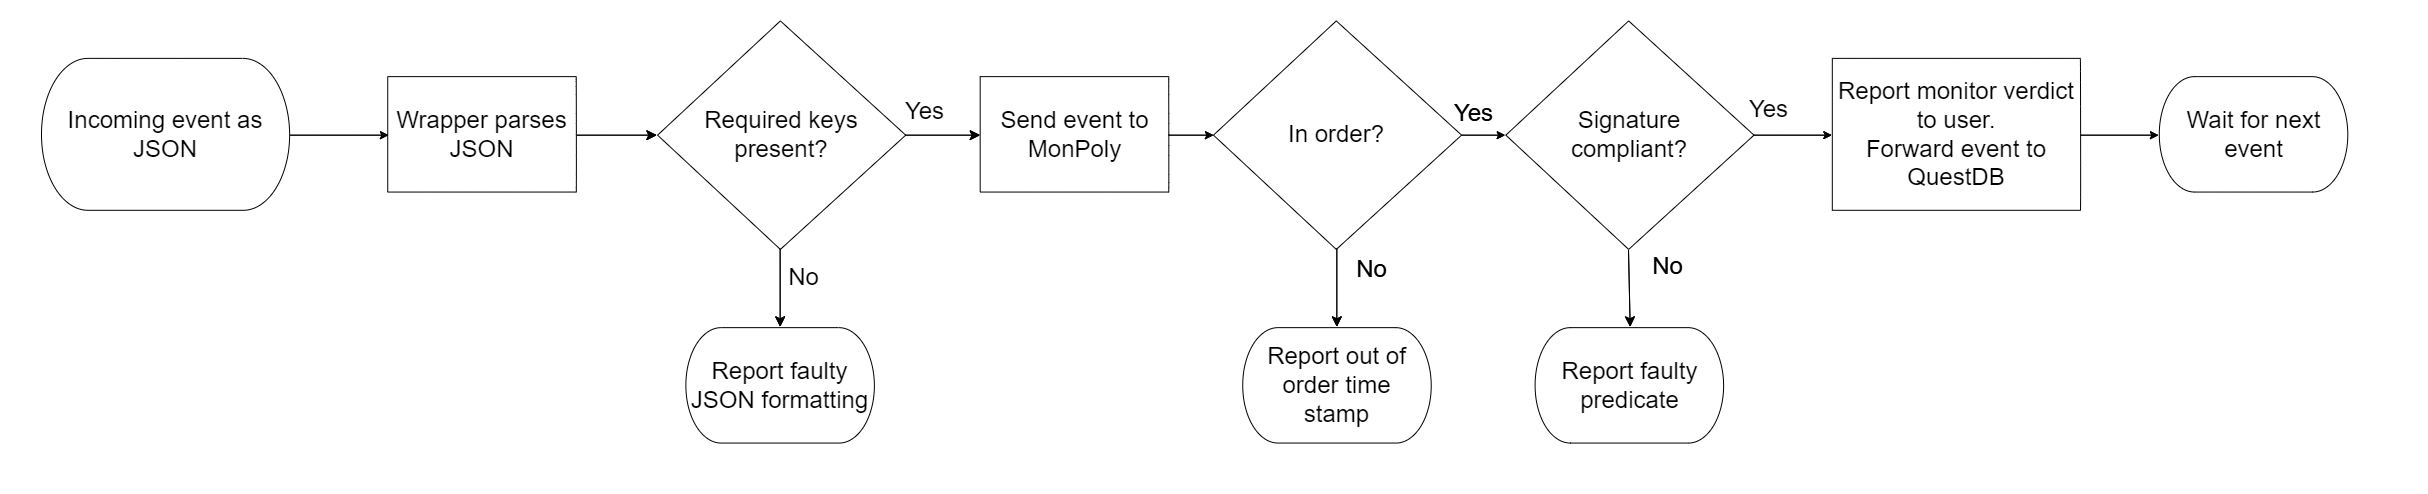
\includegraphics[width=110mm]{diagrams/flowchart.png}
    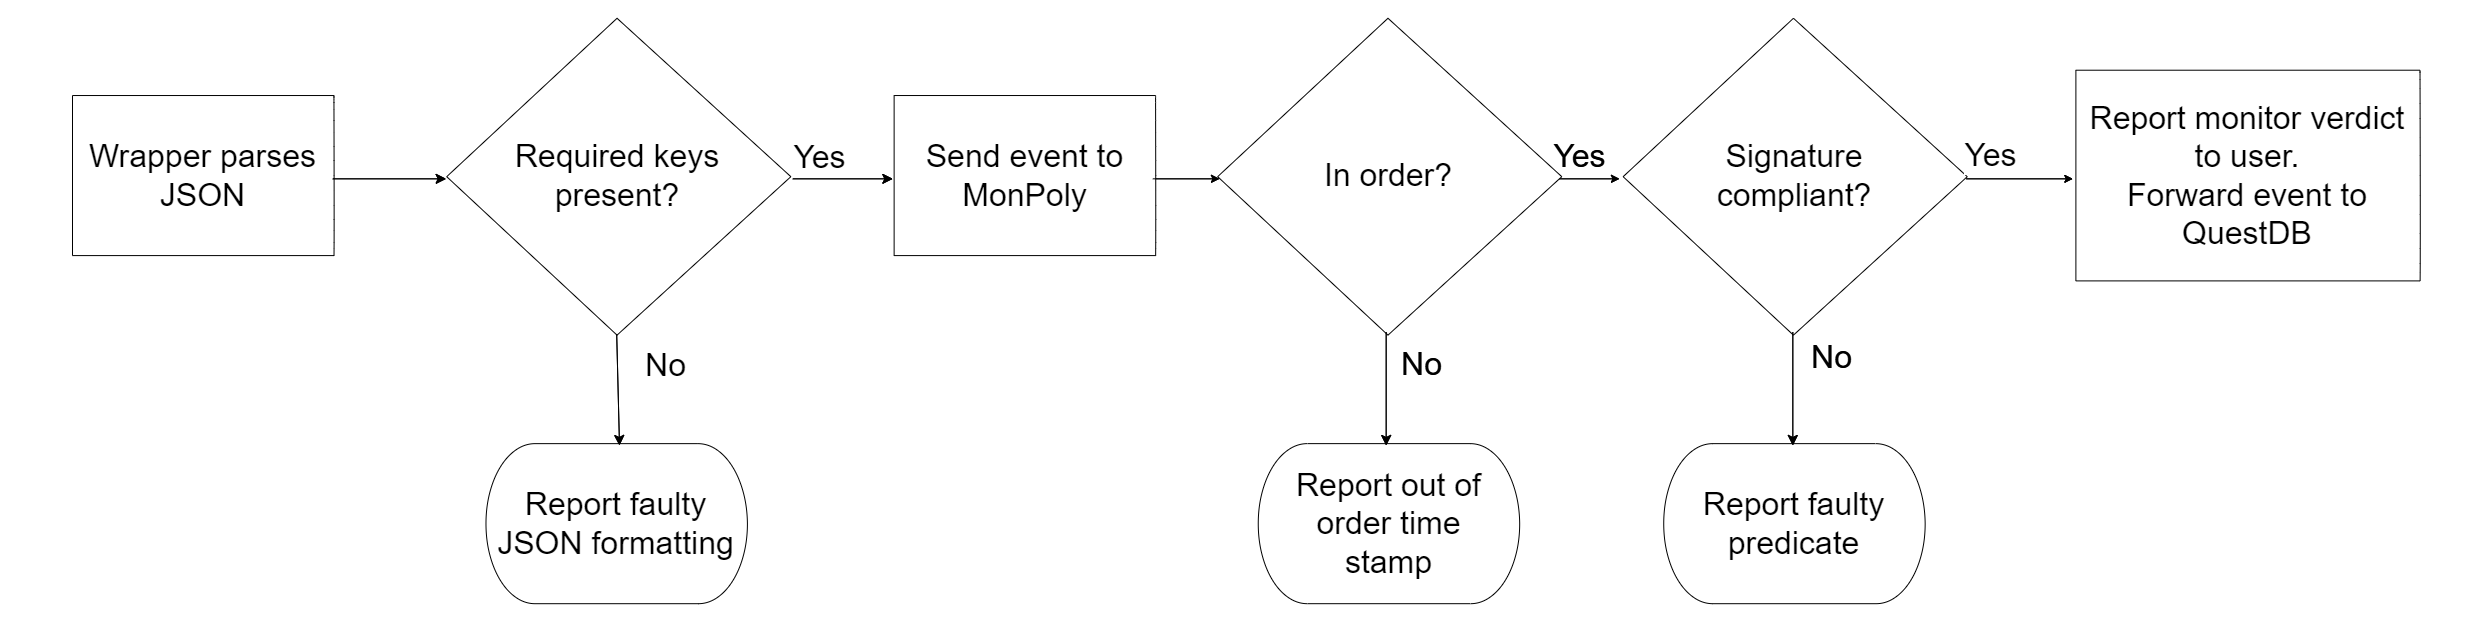
\includegraphics[width=\linewidth]{diagrams/flowchart-2.png}
    \caption{Control flow for an incoming}
\end{figure}

The naive approach to a policy change is simply reloading all events that have ever been seen by the monitor and in turn are in the database.
But we can potentially do much better than this.
An initial improvement is to only load all events in the relative interval of the new policy around the most recent time point.
We apply our idea of extended relative intervals to optimize the performance of this first version a policy change.
This version works by stopping the current MonPoly process and starting a new one.


\section{Additions to MonPoly}
We added two flags to MonPoly that, for a signature file, produce the SQL schema, as previously described, or a representation of the signature in JSON respectively.
Those flags are \texttt{-sql} and \texttt{-sig\_to\_json}.
Their usage is shown in the following example.
\begin{verbatim}
$ monpoly -sql <path/to/signature>
$ monpoly -sig_to_json <path/to/signature>
\end{verbatim}
The flag \texttt{-sql\_drop} works analogous to the \texttt{-sql} flag and produces the SQL statements for "dropping", i.e. deleting the tables in the schema.
\begin{verbatim}
$ monpoly -sql_drop <path/to/signature>
\end{verbatim}

The wrapper needs some kind of feedback when a time point has been processed, in order to return potential feedback to the user.
We added the flag \texttt{-ack\_sep} that can be added when starting to monitor a formula with MonPoly.
A separator is a semicolon.
With this flag, every time the parser reaches a semicolon, an acknowledgment gets sent to stdout.
The wrapper can thus be sure that a time point has been fully processed, and no more waiting is required.

As the wrapper does not perform any check on the names, types, and arity of predicates, we want to avoid that MonPoly exits if the wrapper sends a predicate that is "faulty" in any way.
For this purpose we have added a \texttt{-tolerate\_faulty\_predicates} flag.
This flag makes it so that any time points that contain a predicate with wrong arity and/or types of attributes, get skipped.

Next we made some additions to make MonPoly work better for our policy change method.
By default, MonPoly either runs continuously and reads input from standard input or it processes a log file and terminates once it fully processed all events in the file.
We retrieve a potentially large amount of time points from the database during a policy change.
It is useful if these events could be sent to MonPoly as a file.
But as we want to continue monitoring after processing these past time points, MonPoly cannot terminate at this point.
For this purpose we added the flag \texttt{-switch\_to\_stdin\_after\_log}.
With this flag MonPoly processes a log file and once done with that it awaits new input from standard in.
We are not necessarily interested in all the monitor verdicts of the new policy on all these past time points.
Therefore we added a flag (\texttt{-suppress\_stdout}) that suppresses any potential output while processing the time points in the log file.
The output resumes normally afterwards.

The next three flags that we added concern the relative intervals and the extended relative intervals of formulas.
They are \texttt{-get\_relative\_interval}, \texttt{-relative\_interval\_per\_predicate}, and \texttt{-relative\_interval\_per\_predicate\_json}.
The wrapper uses these commands to know which time points and events must be queried from the QuestDB upon a policy change.

\section{Performance Analysis}
For the performance evaluation of the wrapper there are essentially two angles to take.
\begin{enumerate}
    \item[RQ1]
        The first one is, how large is the overhead for monitoring a policy when using the wrapper compared to using MonPoly directly?
    \item[RQ2]
        The second point of interest is, how much can our optimizations, using extended relative intervals, improve a policy change compared to the naive approach?
\end{enumerate}

\subsection{Wrapper vs. MonPoly}
We expect the wrapper to add a certain time overhead to the monitoring as it performs the same action as MonPoly plus some more things.
We are interested in seeing how much more time these other things add to the total time.
Of course, we aim for it to be as small as possible.

To get an idea of this overhead, we measure the time that the wrapper and MonPoly alone take to process equivalent traces with the same policy and signature for both.
We ran 20 experiments with the same policy.
For every experiment we generated increasingly long traces.
In Figure \ref{fig:monpoly-wrapper-total} we present the average total time that the wrapper and MonPoly respectively took to process the events.
We can see that the wrapper takes increasingly more time, but the growth is linear.
This does not come unexpected.
A constant minimal cost will always come from running the trace through a server.
As an added measurement we sent every time point separately to MonPoly and measured the time for this.
The idea behind this is that in our implementation this is how we forward time points to MonPoly, and we wanted to get an idea how much of the overhead this might explain.
Figure \ref{fig:monpoly-wrapper-per-time-point} shows the same information, but averaged by the number of time points/ length of the trace.
One interesting observation from this graph is the different behavior of MonPoly when processing an entire log file and when receiving individual time points continuously from standard input.
For very few time points it appears that the wrapper is slightly faster than MonPoly per time point.
This probably comes down to sample size.

\begin{figure}
    \centering
    \label{fig:monpoly-wrapper-total}
    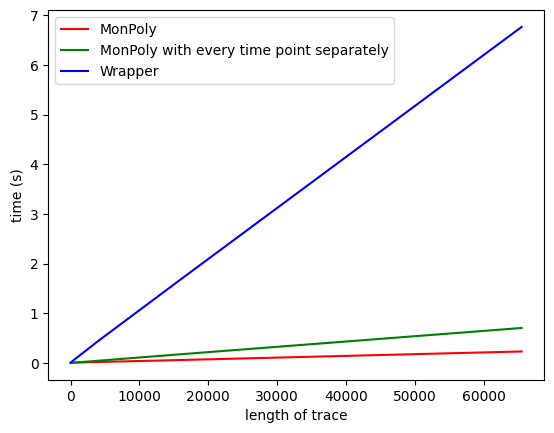
\includegraphics[width=0.8\linewidth]{diagrams/wrapper-monpoly-total.png}
    \caption{Time it takes to process variably long traces}
\end{figure}

\begin{figure}
    \centering
    \label{fig:monpoly-wrapper-per-time-point}
    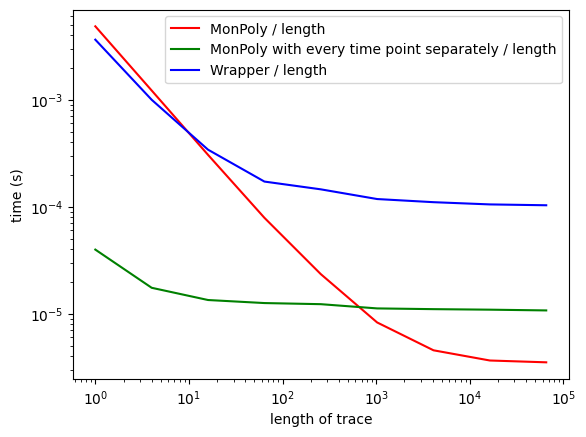
\includegraphics[width=0.8\linewidth]{diagrams/wrapper-monpoly-per-time-point.png}
    \caption{Time it takes to process a trace by the number of time points in the trace}
\end{figure}

\subsection{Policy Change Performance}

In this section we give an idea of the performance of the naive policy change where all events are in the database are processed compared to the performance with our optimization that uses only the events in the extended relative intervals (ERI).

We have compared a policy change using our optimizations to the naive approach by using two random policies and generating random traces of various lengths.
We then compare how the two methods perform for an increasing number of time points.
We have run the same randomized experiment 20 times.
The setup is that we monitor a random policy and measure the time it takes to change the policy after traces with $4^i$, for $i \in [1,9]$, time points have been stored in the database previously.
Figure \ref{fig:policy-change-total} shows the average time it takes to change the policy for both versions of a policy change in respect to the trace length.
Figure \ref{fig:policy-change-per-time-point} shows the same information, but the time has been averaged by time point.
We see that there is large variation for small traces and for a bit the naive change is actually faster, but for large traces our optimization consistently beats the baseline.
From the averaged graph we can't make out much of an improvement.
We do see that both get faster per time point, when there are more total time points.
This can potentially be attributed to amortization costs that have to be paid for a small number as well as for a large number of time points.
Of course the expected performance improvement depends heavily on the formula, if it has large extended relative intervals it is barely different from the naive case, and also on the size of the trace stored in the database.

\begin{figure}
    \centering
    \label{fig:policy-change-total}
    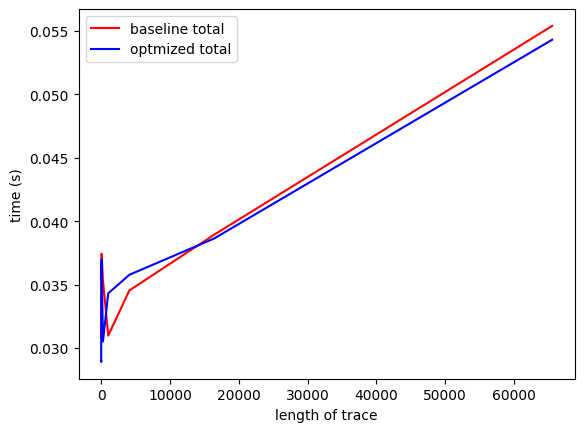
\includegraphics[width=0.8\linewidth]{diagrams/policy-change-total-time.png}
    \caption{Total time a policy change takes for various numbers of time points in a trace}
\end{figure}

\begin{figure}
    \centering
    \label{fig:policy-change-per-time-point}
    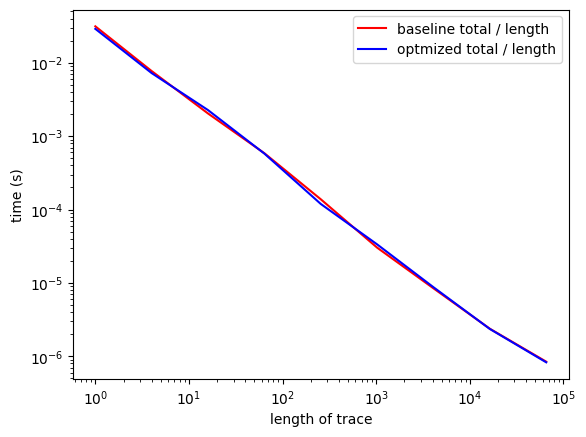
\includegraphics[width=0.8\linewidth]{diagrams/policy-change-time-per-time-point.png}
    \caption{Time it takes to change the policy in respect to the total number of events in the trace}
\end{figure}

\section{Partial Policy Change}

We have started looking into a different method for a policy change that could be done directly through MonPoly and would not rely on the wrapper and the presence of a database.
The general idea is that in many use cases it is common that a policy is made up of many individual parts and one might want to change only a small part of a formula.
Consider for example a privacy policy on a website.
Let's say a user has the ability to specify where their data may and may not be used.
Maybe they had selected very restrictive options, but now want to allow their data to be used in one specific case.
MonPoly has now continuously been monitoring the restrictive policy and also has the state for all the sub-formulas in the larger policy.
In terms of efficiency it would be useful, if the state would only need to be recomputed for the one part that got changed and if the rest of the state could be kept.

One case might be where policies are all in conjunctive normal form (CNF) and single conjuncts might get added or removed.
To remove a conjunct from the formula it needs some sort of identifier.
In a regular structure like a CNF formula this could be done by automatic indexing.
But it still poses some questions, like what happens if the monitor rewrites the formula to an equivalent one, but changes the order.
Then the user doesn't have an inherent idea of a conjuncts' location anymore.
Our solution to this problem was thus to let the user provide identifiers in the form of strings for certain sub-formulas.

We have begun implementing this change in MonPoly.
Our idea makes use of the existing commands feature that lets a user control certain aspects of MonPoly during its runtime.
We envision commands of the form "remove sub-formula x", "add formula y as a conjunct to sub-formula x".
The second example would replace place the sub formula "x and y" in place of "x".
An analogous thing for "or" with an "add disjunct" command is also perceivable.
Or also a command like "negate sub-formula x".

With all this, MonPoly would parse the new formula part, add it to the existing formula, check if the new formula is monitorable, and if so it updates the policy.
Similarly if a part gets removed a check on monitorability of the remaining formula needs to be done.
Before adding a sub-formula, the existing trace has to be checked against that sub-formula and this state must get combined with the pre-existing state of MonPoly.

We have started implementing a feature that allows for named formulas inside MonPoly.
The names should have no effect on the monitoring and solely act as the identifiers of formula parts.
For this we extended \texttt{formula} in MonPoly by an additional type, \texttt{NamedFormula of (string * formula)}.
And similarly we added the type \texttt{ENamedExtf of string * extformula * int} to \texttt{extformula}.

To specify a named (sub)formula in a MonPoly policy, we have extended the formula parser and lexer to accept formulas with the following syntax,
\begin{verbatim}
NAME[f1, name1] AND NAME[f2 OR f3, name2].
\end{verbatim}

